\documentclass[8pt]{beamer}

%%%%%%%%%%%%%%%%%% Extensions %%%%%%%%%%%%%%%%%%%

%\usepackage[table]{xcolor}
\usepackage{amssymb}
\usepackage{amsmath}
\usepackage{amsthm}
\usepackage{array}
\usepackage[T1]{fontenc}
\usepackage[utf8]{inputenc}
\usepackage{layout}


\usepackage{listings}
%\usepackage[margin=2cm]{geometry}
\usepackage{hyperref}

\definecolor{commentgreen}{RGB}{2,112,10}
\definecolor{eminence}{RGB}{108,48,130}
\definecolor{weborange}{RGB}{255,165,0}
\definecolor{frenchplum}{RGB}{129,20,83}
\definecolor{lgrey}{RGB}{235,235,235}

\lstset{
  language=C,                     % choose the language of the code
  numbers=none,                   % where to put the line-numbers
  stepnumber=1,                   % the step between two line-numbers.        
  numbersep=5pt,                  % how far the line-numbers are from the code
  backgroundcolor=\color{lgrey},  % choose the background color. You must add \usepackage{color}
  inputencoding=utf8,
  frame=tb,
  upquote=true,
  commentstyle=\color{commentgreen},
  keywordstyle=\color{eminence},
  stringstyle=\color{red},
  basicstyle=\small\ttfamily, % basic font setting
  emph={int,char,double,float,unsigned,void,bool},
  emphstyle={\color{blue}},
  showspaces=false,               % show spaces adding particular underscores
  showstringspaces=false,         % underline spaces within strings
  showtabs=false,                 % show tabs within strings adding particular underscores
  tabsize=4,                      % sets default tabsize to 2 spaces
  %captionpos=b,                   % sets the caption-position to bottom
  breaklines=false,                % sets automatic line breaking
  breakatwhitespace=true,         % sets if automatic breaks should only happen at whitespace
  title=\lstname,                 % show the filename of files included with \lstinputlisting;
}

%%%%%%%%%%%%%%%%%% Notations %%%%%%%%%%%%%%%%%%%

\newcommand{\nc}{\newcommand}
\nc{\dsp}{\displaystyle}
\nc{\pprime}{\prime\prime}
\nc{\mrm}{\mathrm}
\nc{\lbr}{\lbrack}
\nc{\rbr}{\rbrack}
\nc{\mT}{\mathrm{T}}
\nc{\R}{\mathbb{R}}
\nc{\Z}{\mathbb{Z}}
\nc{\bfx}{\mathbf{x}}
\nc{\bfs}{\mathbf{s}}
\nc{\bfn}{\mathbf{n}}
\nc{\bfe}{\mathbf{e}}
\nc{\ora}{\overrightarrow}
\nc{\Dx}{\Delta x}
\nc{\Dt}{\Delta t}

%%%%%%%%%%%%%%%%%%%%%%%%%%%%%%%%%%%%%%%%%%%%%%%%%
\begin{document}

%%%%%%%%%%%%%%%%%%%%%%%%%%%%%%%%%%%%%%%%%%%%%%%%%%%%%%%%%%%%%%%%%%%%%%%%%%%%%%%
\begin{frame}

\frametitle{About language  ``popularity''}

\begin{center}
 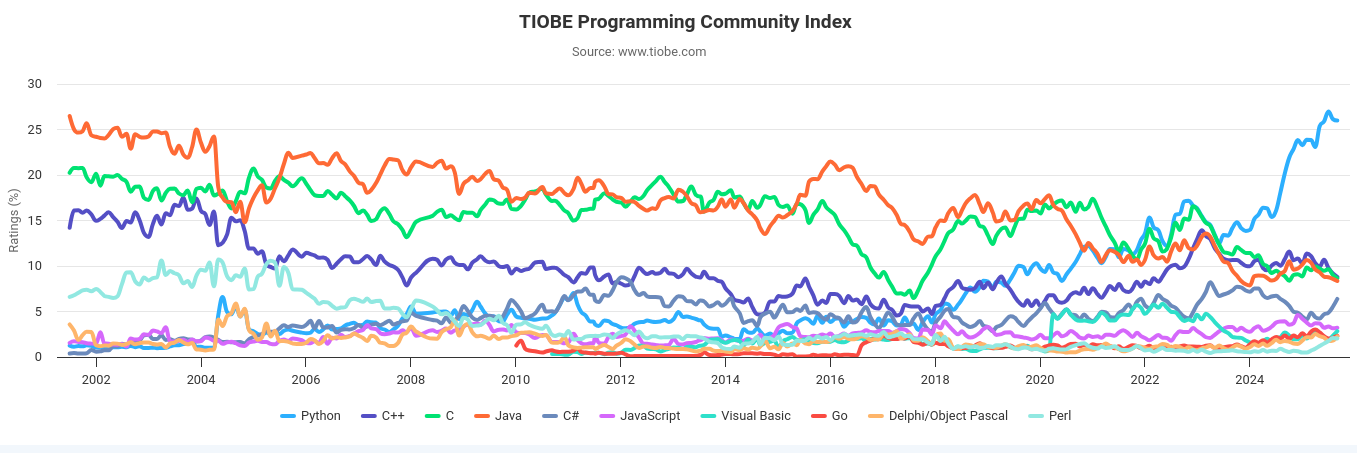
\includegraphics[width=\textwidth]{data/Tiobeindex.png}
\end{center}

\begin{quote}
 There are only two kinds of languages: the ones people complain about and the ones nobody uses. 
(Bjarne Stroustrup, the C++ programming language)
\end{quote}

For scientific programming, a recommended choice today is C/C++ and/or Python.
Development in Python is faster than in C/C++ but doesn't scale well
unless it is used as glue language to interface between existing
compiled code with a C API. 

\end{frame}
%%%%%%%%%%%%%%%%%%%%%%%%%%%%%%%%%%%%%%%%%%%%%%%%%%%%%%%%%%%%%%%%%%%%%%%%%%%%%%%

%%%%%%%%%%%%%%%%%%%%%%%%%%%%%%%%%%%%%%%%%%%%%%%%%%%%%%%%%%%%%%%%%%%%%%%%%%%%%%%
\begin{frame}[containsverbatim]
\frametitle{Compatibility between C and C++}

It is almost but not completely true that C is a subset of C++. When (re)using 
existing C code into a C++ project you'll probably only need to take into
account the following two :

\medskip

\begin{itemize}
	\item C++ has stricter rules for implicit type conversions.
	\item C++ function names are ``mangled'' in compiled object files. 
\end{itemize}

\medskip

We next describe how to take care of these incompatibility; the reasons behind 
these will become clearer later when we describe new features allowed by C++. 

\end{frame}
%%%%%%%%%%%%%%%%%%%%%%%%%%%%%%%%%%%%%%%%%%%%%%%%%%%%%%%%%%%%%%%%%%%%%%%%%%%%%%%


%%%%%%%%%%%%%%%%%%%%%%%%%%%%%%%%%%%%%%%%%%%%%%%%%%%%%%%%%%%%%%%%%%%%%%%%%%%%%%%
\begin{frame}[containsverbatim]
\frametitle{Turning C code into C++ code}

{\bf I. At the level of source code : stricter conversion rules.} \\[3pt]
Contrary to C, in C++ a ({\tt void *}) pointer cannot be 
implicitly cast into other pointer types. 
An important implication concerns {\tt malloc} : code like e.g.
\begin{lstlisting}[caption=]
#include <stdlib.h>
int *p = malloc(10 * sizeof(int));
\end{lstlisting}
should be adapted as
\begin{lstlisting}[caption=]
#include <stdlib.h>
int *p = (int *)malloc(10 * sizeof(int));
\end{lstlisting}
or the more C++-ish
\begin{lstlisting}[caption=]
#include <cstdlib>
int *p = static_cast<int *>(malloc(10 * sizeof(int)));
\end{lstlisting}
It is common to use the equivalent
\begin{lstlisting}[caption=]
#include <cstdlib>
int *p = static_cast<typeof(p)>(malloc(10 * sizeof(*p)));
\end{lstlisting}
so that if one changes mind later and opt for e.g. {\tt float} instead of {\tt int} then 
the change needs only be made in one place.
\end{frame}
%%%%%%%%%%%%%%%%%%%%%%%%%%%%%%%%%%%%%%%%%%%%%%%%%%%%%%%%%%%%%%%%%%%%%%%%%%%%%%%

%%%%%%%%%%%%%%%%%%%%%%%%%%%%%%%%%%%%%%%%%%%%%%%%%%%%%%%%%%%%%%%%%%%%%%%%%%%%%%%
\begin{frame}[containsverbatim]
\frametitle{Turning C code into C++ code}
Note:\\
Later we shall see that one could use the {\tt new} operator instead of the {\tt malloc} function.

\medskip

\begin{lstlisting}[caption=]
int *p = new int[10];
\end{lstlisting}

\medskip

In such a case the call to {\tt free} will be replaced by the {\tt delete}
operator:

\medskip

\begin{lstlisting}[caption=]
delete[] p;
\end{lstlisting}

\medskip

The {\tt new} and {\tt delete} operators are non existing in C.

\medskip

For types more complex than fundamental types (more precisely: POD types, for Plain
Old Data) they have more implications than just memory allocation (call of 
constructors and destructors in particular), so they should not be considered 
equivalent. 

\medskip

Besides, there is no native C++ replacement
for {\tt realloc}.
\end{frame}
%%%%%%%%%%%%%%%%%%%%%%%%%%%%%%%%%%%%%%%%%%%%%%%%%%%%%%%%%%%%%%%%%%%%%%%%%%%%%%%

%%%%%%%%%%%%%%%%%%%%%%%%%%%%%%%%%%%%%%%%%%%%%%%%%%%%%%%%%%%%%%%%%%%%%%%%%%%%%%%
\begin{frame}[containsverbatim]
\frametitle{Turning C code into C++}
{\bf II. Inside header files : avoiding name mangling.} \\[3pt]

If you intend to share your compiled code in the form of object files or shared libraries
in such a way that it can be used with any language with a C API call
capability (many languages do), you sould modify your headers in two 
ways. First they should not contain any 
C++ feature not available in C, and second a safe guard (extern C) 
should be used to prevent from name mangling by the C++ compiler. 

\begin{lstlisting}[caption=]
#pragma once
/* Includes go first as usual */
.
.
.
/* Then C interface statement */
#ifdef __cplusplus
extern "C" {
#endif
/* The bulk of the header goes here */
.
.
.
/* End of C interface */
#ifdef __cplusplus
}
#endif
\end{lstlisting}
\end{frame}
%%%%%%%%%%%%%%%%%%%%%%%%%%%%%%%%%%%%%%%%%%%%%%%%%%%%%%%%%%%%%%%%%%%%%%%%%%%%%%%

%%%%%%%%%%%%%%%%%%%%%%%%%%%%%%%%%%%%%%%%%%%%%%%%%%%%%%%%%%%%%%%%%%%%%%%%%%%%%%%
\begin{frame}[containsverbatim]
\frametitle{Turning C code into C++ code}
{\bf III. At the level of the compiler} :\\[3pt]

You should use a C++ aware compiler...

Inside the GNU family, {\tt g++} should replace {\tt gcc}.

\medskip

It is actually not a bad idea to use {\tt g++} even for C code. 
Since C++ rules regarding types and implicit conversions are stricter, it
can often catch bugs that you may not have noticed otherwise. Turning on all warnings
and debug symbols is recommended in debug builds :

\begin{lstlisting}[caption=]
g++ -Wall -g [...]
\end{lstlisting}

For release builds instead, debug symbols and assertions check should be turned
off, and compiler optimization turned on:

\begin{lstlisting}[caption=]
g++ -DNDEBUG -O3 [...]
\end{lstlisting}

\medskip

If you end-up using CMake (recommended), the distinction is done using either 
\begin{lstlisting}[caption=]
cmake -DCMAKE_BUILD_TYPE=Debug [...]
\end{lstlisting}
or
\begin{lstlisting}[caption=]
cmake -DCMAKE_BUILD_TYPE=Release [...]
\end{lstlisting}

\end{frame}
%%%%%%%%%%%%%%%%%%%%%%%%%%%%%%%%%%%%%%%%%%%%%%%%%%%%%%%%%%%%%%%%%%%%%%%%%%%%%%%

%%%%%%%%%%%%%%%%%%%%%%%%%%%%%%%%%%%%%%%%%%%%%%%%%%%%%%%%%%%%%%%%%%%%%%%%%%%%%%%
\begin{frame}[containsverbatim]
\frametitle{C++ features: References}

References look and taste like pointers, but they are not pointers.

\medskip

The main differences are :

\begin{itemize}
	\item A reference to a variable must always be valid (i.e.
		there is no equivalent of a NULL pointer), and in
		particular it must be initialized by the same time it is
		declared.
	\item A reference cannot be reassigned to refer to another variable than
		the one it was initialized with. Also there is no such thing as
		reference arithmetics, contrary to pointer arithmetics.
	\item A reference can later be used in code exactly as if it was the
		original variable (whereas pointers need to be dereferenced, 
		they have special operators for field access ({\tt ->} instead
		of {\tt .}).
	\item References are introduced by the symbol {\tt \&} rather than {\tt
		*}.
\end{itemize}

They can be understood as {\it aliases} to existing variables.\\[3pt]

\begin{lstlisting}[caption=]
int a;
a = 5;
int &b; /* Syntax error: must be initialized as soon as declared */
int &c = a; /* OK, c is a reference to a */
c = 7;
printf("Value of a : %d\n", a); /* -> Value of a : 7 */
\end{lstlisting}
\end{frame}
%%%%%%%%%%%%%%%%%%%%%%%%%%%%%%%%%%%%%%%%%%%%%%%%%%%%%%%%%%%%%%%%%%%%%%%%%%%%%%%

%%%%%%%%%%%%%%%%%%%%%%%%%%%%%%%%%%%%%%%%%%%%%%%%%%%%%%%%%%%%%%%%%%%%%%%%%%%%%%%
\begin{frame}[containsverbatim]
\frametitle{C++ features: References}

By far the main use of references is {\it pass by reference} of function
arguments. Indeed, recall that C arguments passing is always by copy.

\medskip

Example:\\[3pt]

\begin{lstlisting}[caption=]
int *build_adjacency_table(const struct Mesh& m)
{
	int *adj = (int *)malloc(3 * m.tri * sizeof(int));
	/* Note m.tri, not m->tri */
	[...]
	return adj;
}
\end{lstlisting}

In the above, it is said that the argument $m$ is a reference to a (constant) {\tt struct
Mesh}.

\medskip

In code it could then be used as in

\begin{lstlisting}[caption=]
struct Mesh m;
[...]
int *adj = build_adjacency_table(m); /* Note: m, not &m */
\end{lstlisting}



\end{frame}
%%%%%%%%%%%%%%%%%%%%%%%%%%%%%%%%%%%%%%%%%%%%%%%%%%%%%%%%%%%%%%%%%%%%%%%%%%%%%%%

%%%%%%%%%%%%%%%%%%%%%%%%%%%%%%%%%%%%%%%%%%%%%%%%%%%%%%%%%%%%%%%%%%%%%%%%%%%%%%%
\begin{frame}[containsverbatim]
\frametitle{C++ features: Functions overloading}

In C, a function is characterized (i.e. uniquely determined) by its name.\\


In particular, in C it is not possible to use the same function name for, e.g., 
taking the absolute value of a double and the absolute value of an int. 
For that reason, the standard C library has both the functions
\begin{lstlisting}[caption=]
int abs(int n);
\end{lstlisting}
and
\begin{lstlisting}[caption=]
double fabs(double x);
\end{lstlisting}

It is somewhat inconvient because:
\begin{enumerate}
 \item it is a limitation of expressivity of the language,
 \item it is a possible source of bugs:
 \end{enumerate}
\begin{lstlisting}[caption=]
double a = -0.5;
double b = abs(a);
\end{lstlisting}
This code will compile and the compiler will produce no warning (be it gcc or
g++), even with -Wall. But the resulting value of b is $0$, not $0.5$. This is
not a bug, but a consequence of implicit conversions for arithmetic types.
\end{frame}


%%%%%%%%%%%%%%%%%%%%%%%%%%%%%%%%%%%%%%%%%%%%%%%%%%%%%%%%%%%%%%%%%%%%%%%%%%%%%%%
\begin{frame}[containsverbatim]
\frametitle{C++ features: Functions overloading}
Instead, in C++ a function is characterized by : 
\begin{enumerate}
 \item its name,
 \item the number of its arguments,
 \item the types of its arguments.
\end{enumerate}
Note : Only the types of arguments, {\bf not} the type of its return value.

\medskip

As a consequence, it is valid to declare:

\begin{lstlisting}[caption=]
int abs(int n);
double abs(double x);
\end{lstlisting}

Note that the implemention of both would be indentical except for the types.
Templates (see later) are precisely meant for such situations:

\begin{lstlisting}[caption=]
template <typename T>
T abs(T n)
{
	return n < 0 ? -n : n;
}
\end{lstlisting}
\end{frame}
%%%%%%%%%%%%%%%%%%%%%%%%%%%%%%%%%%%%%%%%%%%%%%%%%%%%%%%%%%%%%%%%%%%%%%%%%%%%%%%

%%%%%%%%%%%%%%%%%%%%%%%%%%%%%%%%%%%%%%%%%%%%%%%%%%%%%%%%%%%%%%%%%%%%%%%%%%%%%%%
\begin{frame}[containsverbatim]
\frametitle{C++ features: Functions overloading}
In the same vein, C++ functions can also have {\it default arguments}. 

\medskip

A function declared as:
\begin{lstlisting}[caption=]
int read_mesh(const char* filename, bool check_integrity = false);
\end{lstlisting}
could be called either as
\begin{lstlisting}[caption=]
read_mesh(filename);
\end{lstlisting}
(in which case {\tt check\_integrity} would be {\tt false}), or e.g. as 
\begin{lstlisting}[caption=]
read_mesh_file(filename, true);
\end{lstlisting}
it which case it would be {\tt true}. Useful when the function is often called with
the default value, and rarely with a different value. Use with parcimony.  

\medskip

There may be more than one argument with a default value, but if there are N of
them they must be the last N arguments of the function.

\medskip

Note: name mangling in object files by the C++ compiler is a consequence a
this function overload feature. A compatible C API should therefore never
use that feature at the level of the interface (it can use it internally though).

\end{frame}
%%%%%%%%%%%%%%%%%%%%%%%%%%%%%%%%%%%%%%%%%%%%%%%%%%%%%%%%%%%%%%%%%%%%%%%%%%%%%%%

%%%%%%%%%%%%%%%%%%%%%%%%%%%%%%%%%%%%%%%%%%%%%%%%%%%%%%%%%%%%%%%%%%%%%%%%%%%%%%%
\begin{frame}[containsverbatim]
\frametitle{C++ features: Methods}

In C++ a method is a function that puts a special emphasize on one of its
argument, of {\tt struct} type. It corresponds to a shift of view point typical
of object oriented programming: objects running methods, instead of functions
applied to objetcs.

\medskip

Example :\\[3pt]

\begin{lstlisting}[caption=]
struct Mesh {
	/* Fields */
	int nvert;
	int ntri;
	struct Vertex *vertices;
	struct Triangle *triangles;
	/* Methods declaration */
	int read_from_file(const char* filename);
	float compute_area() const; 
};
\end{lstlisting}

which could then be used as in 

\begin{lstlisting}[caption=]
struct Mesh m;
m.read_from_file("test.mesh");
double area = m.compute_area();
\end{lstlisting}

\end{frame}
%%%%%%%%%%%%%%%%%%%%%%%%%%%%%%%%%%%%%%%%%%%%%%%%%%%%%%%%%%%%%%%%%%%%%%%%%%%%%%%

%%%%%%%%%%%%%%%%%%%%%%%%%%%%%%%%%%%%%%%%%%%%%%%%%%%%%%%%%%%%%%%%%%%%%%%%%%%%%%%
\begin{frame}[containsverbatim]
\frametitle{C++ features: Methods}

Methods have direct access to the data (and also other methods) of their associated struct.
In the previous example the second method could be defined (it was already declared) as

\begin{lstlisting}[caption=]
double Mesh::compute_area() const
{
	double area = 0;
	for (int i = 0; i < ntri; ++i)
	{
		struct Vertex v1 = vertices[triangles[i].v1];
		struct Vertex v2 = vertices[triangles[i].v2];
		struct Vertex v3 = vertices[triangles[i].v3];
		area += triangle_area(v1, v2, v3);
	}
	return area;
}
\end{lstlisting}
where {\tt triangle\_area} would be a utility function already defined
elsewhere.\\[3pt]

The operator {\tt ::} above is called the {\it resolution} operator. Here it means : the
method {\tt compute\_area} of the struct {\tt Mesh}.\\[3pt]

The {\it free function} equivalent prototype (a free function is a C++ way to refer to a function
which is not a method) would be

\begin{lstlisting}[caption=]
double compute_mesh_area(const struct Mesh &m);
\end{lstlisting}


\end{frame}
%%%%%%%%%%%%%%%%%%%%%%%%%%%%%%%%%%%%%%%%%%%%%%%%%%%%%%%%%%%%%%%%%%%%%%%%%%%%%%%

%%%%%%%%%%%%%%%%%%%%%%%%%%%%%%%%%%%%%%%%%%%%%%%%%%%%%%%%%%%%%%%%%%%%%%%%%%%%%%%
\begin{frame}[containsverbatim]
\frametitle{C++ features: Constructors and Destructors}

Constructors (resp. destructors) are special methods that are implicitely 
(if not explicitely) called when an instance of a struct enters (resp. leaves) 
the current scope in the code.\\


\medskip

They are typically used to initialize the struct fields or process with
some memory allocation, for constructors, and for clean-up, for destructors.

\medskip

They must have special names: constructors are named identically to their 
corresponding struct name, and destructors names are the struct name with
a $\sim$ in front.

\medskip

(Following code refer to the didiersmets/Myosotis github repo)\\
Example  : (show and comment include/array.h  and then include/hash\_table.h)



\end{frame}
%%%%%%%%%%%%%%%%%%%%%%%%%%%%%%%%%%%%%%%%%%%%%%%%%%%%%%%%%%%%%%%%%%%%%%%%%%%%%%%

%%%%%%%%%%%%%%%%%%%%%%%%%%%%%%%%%%%%%%%%%%%%%%%%%%%%%%%%%%%%%%%%%%%%%%%%%%%%%%%
\begin{frame}[containsverbatim]
\frametitle{C++ features: Operators overloading}

(show and comment include/vec3.h)



\end{frame}
%%%%%%%%%%%%%%%%%%%%%%%%%%%%%%%%%%%%%%%%%%%%%%%%%%%%%%%%%%%%%%%%%%%%%%%%%%%%%%%

%%%%%%%%%%%%%%%%%%%%%%%%%%%%%%%%%%%%%%%%%%%%%%%%%%%%%%%%%%%%%%%%%%%%%%%%%%%%%%%
\begin{frame}[containsverbatim]
\frametitle{C++ features: Derived structs and inheritance}

(show and comment include/vertex\_table.h)

\end{frame}
%%%%%%%%%%%%%%%%%%%%%%%%%%%%%%%%%%%%%%%%%%%%%%%%%%%%%%%%%%%%%%%%%%%%%%%%%%%%%%%

\end{document}

